\documentclass[12pt]{article}
\pagestyle{empty}
\usepackage{amsmath,times,bm,hyperref}
\usepackage{amssymb}
\usepackage{stmaryrd}
\usepackage{graphicx}
\usepackage{listings}
\usepackage{xcolor}
\lstset { %
    language=C++,
    backgroundcolor=\color{black!5}, % set backgroundcolor
    basicstyle=\footnotesize,% basic font setting
}

%%%%%%%%%%%%%%%%%%%%%%%%%%%%%%%%%%%%%%%%%%%%%%%%%%
% Do not modify the dimensions of the page
\setlength{\topmargin}{0mm}
\setlength{\headheight}{0mm}
\setlength{\headsep}{0mm}
%% 25.4 -25.4 = 0
\setlength{\topmargin}{0mm}
%% 25.4 -25.4 = 0
\setlength{\oddsidemargin}{0mm}
%% 210 -25(left) -25(right) = 160
\setlength{\textwidth}{160mm}
%% 297 -25(top) -30(bottom) = 242
\setlength{\textheight}{242mm}
\setlength{\parindent}{0pt}
\setlength{\parskip}{12pt}
% Do not modify the dimensions of the page
%%%%%%%%%%%%%%%%%%%%%%%%%%%%%%%%%%%%%%%%%%%%%%%%%%

\begin{document}

\begin{center}
% TITLE: replace text with your abstract title WITHOUT full stop
\textbf{\Large
Homework 4
}\\
\normalsize Due April 27 2021

% AUTHOR/AFFILIATION: handled by authblk. 
% Use only one of the two following methods for author listing. Delete or comment out the other.
% Add/remove authors/affiliations as necessary, complete following the template without adding additional superscript/footnotes  

% 1- Authors have the same affiliation:
% ~~~~~~~~~~~~~~~~~~~~~~~~~~~~~~~~~~~~


%%%%% AFFILIATIONS %%%%%

\end{center}
\begin{enumerate}
\item Show that the stiffness matrix of the linear elastostatic problem is symmetric.

\item (Triangle element) Consider the two-dimensional triangle element. Its parent or reference element is defined in the $r-s$ coordinate as is shown in Figure \ref{fig:tri}. For convenience, the coordinate $t := 1 - r - s$ is introduced. It can be easily observed that $t= \mathrm{constant}$ represents the lines parallel to the inclined edge of the triangle.

\begin{figure}[h]
	\begin{center}
	\begin{tabular}{c}
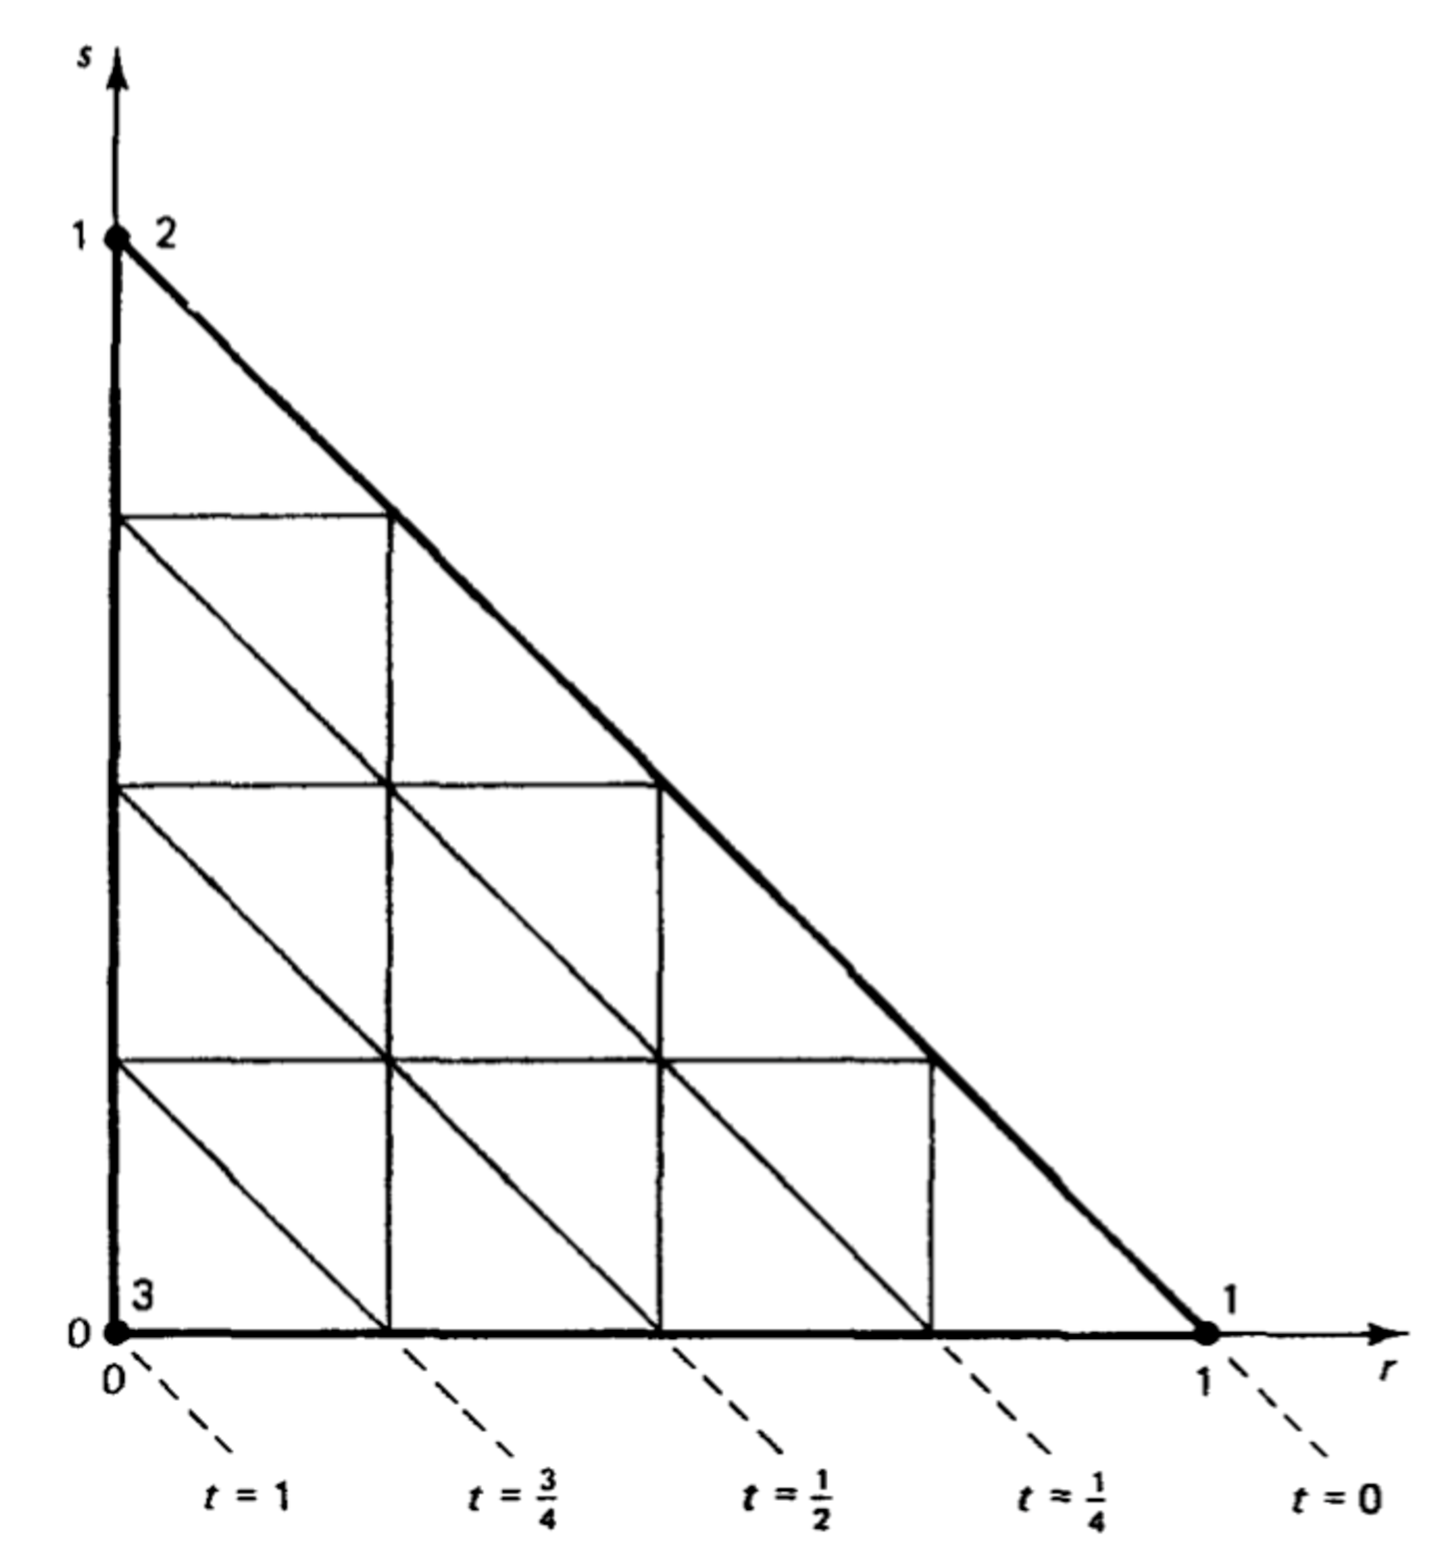
\includegraphics[angle=0, trim=0 0 0 0, clip=true, scale = 0.35]{./triangle_elem.pdf}
\end{tabular}
\end{center} 
\caption{Triangle element in the reference domain.}
\label{fig:tri}
\end{figure}

\begin{enumerate}
\item Consider the three node triangle element, whose shape functions are 
\begin{align*}
N_1(r,s) = r, \quad N_2(r,s) = s, \quad N_3(r,s) = t = 1 - r - s.
\end{align*}
Use the surf function in MATLAB to visualize the shape functions.

\item The quadratic element defined on the triangle has shape functions
\begin{align*}
& N_1(r,s) = r(2r-1), \quad N_2(r,s) = s(2s-1), \quad N_3(r,s) = t(2t-1), \\
& N_4(r,s) = 4rs, \quad N_5(r,s) = 4st, \quad N_6(r,s) = 4rt.
\end{align*}
Again, visualize these shape functions.

\item Consider the 3-point quadrature rule for the triangle shown in Figure \ref{fig:tri} as follows.
\begin{align*}
&w_1 = \frac{1.0}{3.0}, \quad r_1 = 0.5, \quad s_1 = 0.5; \\
&w_2= \frac{1.0}{3.0}, \quad r_2 = 0.5, \quad s_2 = 0.0;\\
&w_3 = \frac{1.0}{3.0}, \quad r_3 = 0.0, \quad s_3 = 0.5.
\end{align*}
Determine the algebraic accuracy of this quadrature rule.
\end{enumerate}



\item (convergence rate of the error in the $L_2$-norm) Revisit the MATLAB code we developed in the second homework and do the following.
\begin{enumerate}
\item Plot the basis functions for polynomial degree 1, 2, 3, 4, 5, and 6 on the reference or parent domain $\hat{\Omega}=[-1,1]$.
\item Let $e:=u^h - u$ be the error in the finite element approximation. Calculate
\begin{align*}
\|e\|_0 := \left( \int_0^1  e^2 dx \right)^{\frac12},
\end{align*}
and 
\begin{align*}
\|u\|_0 := \left( \int_0^1  u^2 dx \right)^{\frac12},
\end{align*}
for meshes with 4, 6, 8, 10, 12, and 16 elements. Report the relative errors $\|e\|_0/\|u\|_0$ for linear, quadratic, cubic, quartic, quintic, and sextic elements in a table. Observe the pattern of the errors and make comments.
\item For the polynomial degree being 1, 2, 3, 4, 5, and 6, tune the number of quadrature points. You may see that the stiffness matrix may be rank deficient (i.e. singular) if there are not enough quadrature points. How many quadrature points are needed to ensure the stiffness to be non-singular for different polynomial degrees? Do you have a theoretical explanation?
\end{enumerate}
\end{enumerate}

\end{document}